\subsection*{Solution to Spring 2007, \#1}\label{s071}
\subsubsection*{Solution to $(i)$}
We compute
\begin{align*}
\lim_{\vep \rightarrow 0}\frac{1}{\vep}(E[u + \vep v] - E[u]) &= \lim_{\vep \rightarrow 0}\frac{1}{\vep}\bigg(\frac{1}{2}\int (f - u - \vep v)^{2}\, dx \\
&\hspace{0.5in}+ \frac{\ld}{2}\int (\Delta u + \vep \Delta v)^{2}\, dx - \frac{1}{2}\int (f - u)^{2}\, dx - \frac{\ld}{2}\int (\Delta u)^{2}\, dx\bigg)\\
&=\int -v(f - u)\, dx + \int \ld \Delta u\Delta v\, dx\\
&= -\int v(f - u)\, dx - \ld\int \del(\lap u)\cdot \del v \, dx\\
&= -\int v(f - u)\, dx + \ld \int (\lap^{2}u)v\, dx.
\end{align*}
Thus the minimizer $u$ satisfies $$0 = -(f - u) + \ld \Delta^{2}u.$$
\hfill\qed

\subsubsection*{Solution to $(ii)$}
Let $T^{2} = [0, 2\pi]^{2}$. We have
\begin{align*}
u(x, y) &= \sum_{(m, n) \in \Z^2}\wh{u}(m, n)e^{i(mx + ny)}\\
\wh{u}(m, n) &= \frac{1}{4\pi^{2}}\int_{T^{2}}u(x, y)e^{-i(mx + ny)}\, dx\, dy.
\end{align*}
Therefore
\begin{align*}
0 &= -(\wh{f}(m, n) - \wh{u}(m, n)) + \ld(-m^{2} - n^{2})^{2}\wh{u}(m, n)\\
0 &= -\wh{f}(m, n) + \wh{u}(m, n) + \ld(m^{2} + n^{2})^{2}\wh{u}(m, n)\\
\wh{u}(m, n) &= \frac{\wh{f}(m, n)}{1 + \ld(m^{2} + n^{2})^{2}}.
\end{align*}
Thus
$$u(x, y) = \sum_{(m, n) \in \Z^{2}}\frac{\wh{f}(m, n)}{1 + \ld(m^{2} + n^{2})^{2}}e^{i(mx + ny)}.$$
\hfill\qed

\subsubsection*{Solution to $(iii)$}
A large $\ld$ decrease the strength of high frequency modes (which correspond to large $m, n$). Smoothness of $u$
is equivalent to rapid decay of Fourier coefficients and so, large values of $\ld$ make $u$ more smooth.
\hfill\qed

\subsection*{Solution to Spring 2007, \#2}\label{s072}
We recall that $\lap u = \frac{1}{r}u_{r} + u_{rr} + \frac{1}{r^{2}}u_{\ta\ta}$.
We break the problem up into
\begin{enumerate}[$(1)$]
\item $\Delta u_{1} = r\cos \ta$ in $\D$, $\displaystyle \frac{\pr u_{1}}{\pr r} = 0$ on $\pr \D$
\item $\Delta u_{2} = 0$ in $\D$, $\displaystyle \frac{\pr u_{2}}{\pr r} = \sin \ta$ on $\pr D$.
\end{enumerate}
Then $u = u_{1} + u_{2}$ satisfies
\begin{align*}
\Delta u = r\cos \ta & \text{ in $\D$}\\
\frac{\pr u}{\pr r} = \sin \ta & \text{ on $\pr \D$.}
\end{align*}
We consider the first problem. Let $u^{1} = ar^{3}\cos\ta$. Then
\begin{align*}
u_{r}^{1} &= 3ar^{2}\cos\ta\\
u_{rr}^{1} &= 6ar\cos\ta\\
u_{\ta}^{1} &= -ar^{3}\sin\ta\\
u_{\ta\ta}^{1} &= -ar^{3}\cos\ta.
\end{align*}
Thus $\Delta u' = r\cos\ta$ is the same as
$$ru_{r}^{1} + r^{2}u_{rr}^{1} + u_{\ta\ta} = r^{3}\cos\ta$$
and substituting the above computations yields that $8a = 1$ and hence $a = 1/8$.
Since $\frac{\pr u^{1}}{\pr r} = \frac{3}{8}\cos\ta$ on $r = 1$,
take $$u_{1} = \frac{1}{8}r^{3}\cos\ta - \frac{3}{8}r\cos\ta.$$
Now we consider the second problem. Let $u_{2} = r\sin\ta$. Then $\Delta u_{2} = 0$ in $\D$ and $\frac{\pr u_{2}}{\pr r} = \sin\ta$ on $\pr\D$.
Thus
\begin{align}\label{s072eq1}
u = \frac{1}{8}r^{3}\cos\ta - \frac{3}{8}r\cos\ta + r\sin\ta = \frac{1}{8}(x^{2} + y^{2})x - \frac{3}{8}x + y
\end{align}
satisfies the desired PDE. We claim that any other solution differs from $u$ as in \eqref{s072eq1} by a constant. Let $v$ be another solution and consider
$w := u - v$. Then
$$\Delta w = 0 \text{ in $\D$, }\quad \frac{\pr w}{\pr n} = 0 \text{ in $\pr\D$.}$$
We have
$$0 = \int_{\D}w\Delta w\, dx = -\int_{\D}\abn{\nabla w}^{2}\, dx + \int_{\pr\D}\frac{\pr w}{\pr n}w\, d\sigma = -\int_{\D}\abn{\nabla w}^{2}\, dx.$$
Thus $\abn{\nabla w} = 0$ on $\D$ and hence $w$ is a constant. Therefore all solutions to
\begin{align*}
\Delta u = x & \text{ in } x^{2} + y^{2} < 1\\
\frac{\pr u}{\pr r} = y & \text{ on } x^{2} + y^{2} = 1
\end{align*}
are $$u(x, y) = \frac{1}{8}(x^{2} + y^{2})x - \frac{3}{8}x + y + C.$$
\hfill\qed

\subsection*{Solution to Spring 2007, \#3}\label{s073}
We will assume that the boundary conditions are of the form
$a(x)u(x, 0, t) + b(x)v(x, 0, t) = 0$ and that $u(x, y, 0)$, $v(x, y, 0)$
are compactly supported. Then by Spring 2008, \#3, $u$ and $v$ are compactly supported.
We have
$$E(t) = \int_{-\infty}^{\infty}\int_{0}^{\infty}u(x, y, t)^{2} + v(x, y, t)^{2}\, dy\, dx$$
and hence
$$\dot{E}(t) = \int_{-\infty}^{\infty}\int_{0}^{\infty}2uu_{t} + 2vv_{t}\, dy\, dx.$$
Note that since
$$\vct{u}{v}_{t} = \pmat{1}{}{}{-1}\vct{u}{v}_{x} + \pmat{}{1}{1}{}\vct{u}{v}_{y}$$
we have
$u_{t} = u_{x} + v_{y}$ and $v_{t} = -v_{x} + u_{y}$.
Thus
\begin{align*}
\dot{E}(t) &= 2\int_{-\infty}^{\infty}\int_{0}^{\infty}u(u_{x} + v_{y}) + v(-v_{x} + u_{y})\, dy\, dx = 2\int_{-\infty}^{\infty}\int_{0}^{\infty}uu_{x} - vv_{x} + uv_{y} + vu_{y}\, dy\, dx\\
&=2\int_{-\infty}^{\infty}\bigg(\int_{0}^{\infty}uu_{x} - vv_{x}\, dy\bigg) - u(x, 0, t)v(x, 0, t)\, dx\\
& = 2\int_{0}^{\infty}\int_{-\infty}^{\infty}uu_{x} - vv_{x}\, dx\, dy - 2\int_{-\infty}^{\infty}u(x, 0, t)v(x, 0, t)\, dx\\
&= 2\int_{0}^{\infty}\bigg(\frac{u^{2}}{2} - \frac{v^{2}}{2}\bigg)\bigg|_{x = -\infty}^{\infty}\, dy - 2\int_{-\infty}^{\infty}u(x, 0, t)v(x, 0, t)\, dx\\
&= -2\int_{-\infty}^{\infty}u(x, 0, t)v(x, 0, t)\, dx = -2\int_{-\infty}^{\infty}u(x, 0, t)^{2}(-\frac{a(x)}{b(x)})\, dx = \int_{-\infty}^{\infty}\frac{a(x)}{b(x)}u(x, 0, t)^{2}\, dx.
\end{align*}
Thus all the $a, b$ such that $\int_{-\infty}^{\infty}\frac{a(x)}{b(x)}u(x, 0, t)^{2}\, dx = 0$ gives all the boundary
conditions of the form $a(x)u(x, 0, t) + b(x)v(x, 0, t) = 0$ such that $E(t)$ remains constant.

All the $a, b$ such that $\int_{-\infty}^{\infty}\frac{a(x)}{b(x)}u(x, 0, t)^{2}\, dx \leq 0$ gives all the boundary conditions
of the form $a(x)u(x, 0, t) + b(x)v(x, 0, t) = 0$ such that $E(t)$ does not increase (the condition is certainly satisfied if
$a(x)/b(x) \leq 0$ for all $x$, but $a(x)/b(x)$ does not need to satisfy this to satisfy $\int_{-\infty}^{\infty}\frac{a(x)}{b(x)}u(x, 0, t)^{2}\, dx \leq 0$).
\hfill\qed

\subsection*{Solution to Spring 2007, \#4}
We have
\begin{align*}
\lap(\abn{\del u}^{2}) &= \lap(\sum_{i = 1}^{d}u_{x_{i}}^{2} = \sum_{j = 1}^{d}\frac{\pr^{2}}{\pr x_{j}^{2}}(\sum_{i = 1}^{d}u_{x_{i}}^{2}) = \sum_{j = 1}^{d}\pr_{x_{j}}\sum_{i = 1}^{d}\pr_{x_{j}}u_{x_{i}}^{2} = \sum_{j = 1}^{d}\pr_{x_{j}}\sum_{i = 1}^{d}2u_{x_{i}}u_{x_{i}x_{j}}\\
& = 2 \sum_{j = 1}^{d}\sum_{i = 1}^{d}u_{x_{i}x_{j}}u_{x_{i}x_{j}} + u_{x_{i}}u_{x_{i}x_{j}x_{j}} = 2\sum_{j = 1}^{d}\sum_{i = 1}^{d}u_{x_{i}x_{j}}^{2} + 2(\del u \cdot \del(\lap u)) \geq 0
\end{align*}
since $\lap u = 0$. Therefore $\abn{\del u}^{2}$ is subharmonic and hence the maximum value in $\ov{D}$ must occur on the boundary of $D$.
\hfill\qed

\subsection*{Solution to Spring 2007, \#5}
\subsubsection*{Solution to $(a)$}
We have
\begin{align*}
u_{t} + 2uu_{x} &= au^{2}\\
u(x, 0) = f(x) &=
\begin{cases}
0 & \text{ if } x < - 1\\
1 + x & \text{ if } -1 < x < 0\\
1 - x & \text{ if } 0 < x < 1\\
0 & \text{ if } x > 1.
\end{cases}
\end{align*}
We use method of characteristics. We have
$$F(p, q, z, x, t) = q + 2zp - az^{2}$$
and
\begin{align*}
\begin{array}{cc}
\dot{x} = 2z & x(0) = x_{0}\\
\dot{t} = 1 & t(0) = 0\\
\dot{z} = az^{2} & z(0) = f(x_{0})
\end{array}
\end{align*}
and hence
$$z(s) = \frac{1}{\frac{1}{f(x_{0})} - as}$$ and $t(s) = s$. Therefore
$$\dot{x}(s) = -\frac{2}{as - \frac{1}{f(x_{0})}} = \frac{-2/a}{s - \frac{1}{af(x_{0})}}$$
which implies that
$$x(s) = -\frac{2}{a}\ln|s - \frac{1}{af(x_{0})}| + x_{0} - \frac{2}{a}\ln|af(x_{0})|.$$
Thus
$$u(x, t) = \frac{1}{\frac{1}{f(y)} - at} := w(y, t)$$
where
\begin{align*}
x &= -\frac{2}{a}\ln|t - \frac{1}{af(y)}| + y - \frac{2}{a}\ln|af(y)|\\
 &= -\frac{2}{a}\ln|atf(y) - 1| + y := x(y, t).
\end{align*}
\hfill\qed

\subsubsection*{Solution to $(b)$}
If $y < -1$, then $f(y) = 0$ and $w(y, t)$ is finite for all time. If $-1 < y < 0$, then $f(y) = 1 + y$. Therefore
$w(y, t)$ is finite for all time $t < \frac{1}{a(1 + y)}$. Since $\inf_{-1 < y < 0}\frac{1}{a(1 + y)} = \frac{1}{a}$,
$w(y, t)$ is finite for all $y \in (-1, 0)$ and $t < 1/a$.

If $0 < y < 1$, then $f(y) = 1 - y$. Therefore $w(y, t)$ is finite for all time $t < \frac{1}{a(1 - y)}$. Since $\inf_{0 < y < 1}\frac{1}{a(1 - y)} = \frac{1}{a}$,
$w(y, t)$ is finite for all $y \in (0, 1)$ and $t < 1/a$.

If $y > 1$, then $f(y) = 0$ and so $w(y, t)$ is finite for all time and $y \in (1, \infty)$.
Thus $w(y, t)$ is finite for $0 \leq t < t^{\ast} = 1/a$ for all $y \in \R$.
\hfill\qed

\subsubsection*{Solution to $(c)$}
For $t \in [0, 1/a)$,
$$x = -\frac{2}{a}\ln(1 - atf(y)) + y.$$
Let $G(x, y, t) := -\frac{2}{a}\ln(1 - atf(y)) + y - x$. Then $G(x, y, t) = 0$.
Since
\begin{align*}
G_{y}(x, y, t) = \frac{2}{a}\frac{1}{1 - atf(y)}atf'(y) + 1 = \frac{2tf'(y)}{1 - atf(y)} + 1 =
\begin{cases}
1 & \text{ if } \abn{y} > 1\\
\frac{2t}{1 - atf(y)} + 1 & \text{ if } -1 < y < 0\\
\frac{-2t}{1 - atf(y)} + 1 & \text{ if } 0 < y < 1.
\end{cases}
\end{align*}
Thus $G_{y}(x, y, t) \neq 0$ for either $|y| > 1$ or $-1 < y < 0$ and $1/a$.
%
%
%
%
\begin{center}
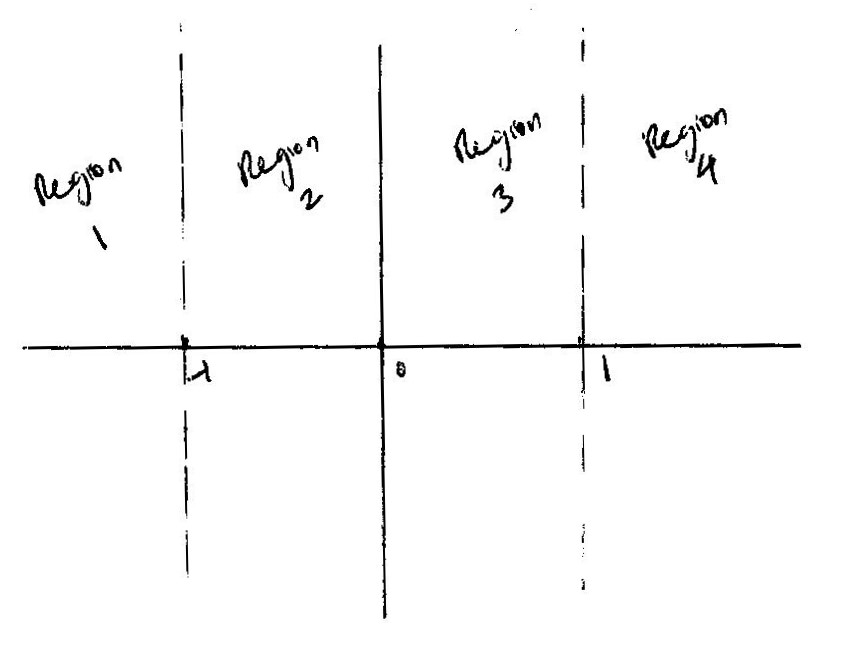
\includegraphics[scale = 0.75]{./_Figures/S07Q5c.jpg}
\end{center}
%
%
%
Thus characteristics don't cross before time $t = 1/a$ for characteristics that start in Regions 1, 2, and 4.
Consider two characteristics that start at $y_{1}$ and $y_{2}$ with $y_{1}, y_{2} \in (0, 1)$. We want to compute
when they crash. (In more ``traditional" notation for method of characteristics, $y_{1}$ is our $(x_{0})_{1}$ and $y_{2}$ is our $(x_{0})_{2}$.)
We want to solve for $t$ in
\begin{align*}
-\frac{2}{a}\ln(1 - at(1 - y_{1})) + y_{1} &= -\frac{2}{a}\ln(1 - at(1 - y_{2})) + y_{2}\\
\frac{2}{a}\ln\frac{1 - at(1 - y_{2})}{1 - at(1 - y_{1})} &= y_{2} - y_{1}\\
1 - at(1 - y_{2}) &= e^{\frac{a}{2}(y_{2} - y_{1})}(1 - at(1 - y_{1}))
\end{align*}
and hence the time when two characteristics that start at $y_{1}$ and $y_{2}$ with $y_{1}, y_{2} \in (0, 1)$ crash is
$$t = \frac{1 - e^{\frac{a}{2}(y_{2} - y_{1})}}{-ae^{\frac{a}{2}(y_{2} - y_{1})}(1 - y_{1}) + a(1 - y_{2})}.$$
Now let $y_{2} = 1/(na)$. Then
\begin{align*}
\lim_{y_{1} \rightarrow 1/(na)}&\frac{1 - e^{\frac{a}{2}(y_{2} - y_{1})}}{a(1 - y_{2}) - ae^{\frac{a}{2}(y_{2} - y_{1})}(1 - y_{1})} = \lim_{y_{1} \rightarrow 1/(na)}\frac{-e^{\frac{a}{2}(y_{2} - y_{1})}(-\frac{a}{2})}{-ae^{\frac{a}{2}(y_{2} - y_{1})}(-\frac{a}{2})(1 - y_{1}) - ae^{\frac{a}{2}(y_{2} - y_{1})}(-1)}\\
&= \lim_{y_{1} \rightarrow 1/(na)}\frac{a/2}{\frac{a^{2}}{2}(1 - \frac{1}{na}) + a} = \frac{a}{a^{2}(1 - \frac{1}{na}) + a} = \frac{1}{a + (1 - \frac{1}{n})} < \frac{1}{a}.
\end{align*}
Now choose $n$ sufficiently large such that $1/(na) < 1$.
Then the above argument shows that if we have a characteristic that starts at $1/(na)$ and another one that starts arbitrarily close,
then these two characteristics crash before time $1/a$. Therefore we cannot solve for $x = x(y, t)$
for all time in $[0, 1/a)$.
\begin{rem}
The technique of analyzing two arbitrarily close characteristics and computing when they crash is crucial to solving
Fall 2015, \#8. \hfill\qed
\end{rem}

\subsection*{Solution to Spring 2007, \#6}
We omit the solution to Problem $6(d)$.
\subsubsection*{Solution to $(a)$}
We have
$$-Cu + u^{3} - u^{2} + u''' = C_{1}.$$
Then
\begin{align*}
-Cu_{r} + u_{r}^{3} - u_{r}^{2} &= C_{1}\\
-Cu_{\ell} + u_{\ell}^{3} - u_{\ell}^{2} &= C_{1}.
\end{align*}
Thus
\begin{align*}
-Cu_{r} + Cu_{\ell} + u_{r}^{3} - u_{\ell}^{3} - u_{r}^{2} + u_{\ell}^{2} &= 0\\
-C(u_{r} - u_{\ell}) + (u_{r} - u_{\ell})(u_{r}^{2} + u_{r}u_{\ell} + u_{\ell}^{2}) - (u_{r} - u_{\ell})(u_{r} + u_{\ell}) &= 0.
\end{align*}
Since $u_{r} \neq u_{\ell}$,
$$-C + (u_{r}^{2} + u_{r}u_{\ell} + u_{\ell}^{2}) - (u_{r} + u_{\ell}) = 0$$
and hence
$$C = (u_{r}^{2} + u_{r}u_{\ell} + u_{\ell}^{2}) - (u_{r} + u_{\ell}).$$
\hfill\qed

\subsubsection*{Solution to $(b)$}
We have
$$C_{1} = -u_{r}(u_{r}^{2} + u_{r}u_{\ell} + u_{\ell}^{2}) + u_{r}(u_{r} + u_{\ell}) + u_{r}^{3} - u_{r}^{2}.$$
Note that this will also give a condition relating $u_{\ell}$ and $u_{r}$ since we can also use the equation relating
$u_{\ell}$ with $C_{1}$ in part $(a)$ to get a (slightly) different expression for $C_{1}$ and these two different expressions
of $C_{1}$ must be equal.
\hfill\qed

\subsubsection*{Solution to $(c)$}
The system can be written as $x' = y$, $y' = z$, $z' = C_{1} + Cx - x^{2} + x^{2}$. The equilibrium points occur
at $\{(a, 0, 0): a^{3} - a^{2} - Ca - C_{1} = 0\}$.
\hfill\qed

\subsection*{Solution to Spring 2007, \#7}
This problem is a good illustration of using integration by parts to obtain decay in integral expressions.
We will assume $\phi$ to be smooth (otherwise we cannot obtain such nice decay).

\subsubsection*{Solution to $(a)$}
We observe that
$$\frac{d}{dx}e^{ik\phi(x)} = e^{ik\phi(x)}ik\phi'(x)$$
and hence
\begin{align}\label{s077star}
\frac{1}{ik\phi'(x)}\frac{d}{dx}e^{ik\phi(x)} = e^{ik\phi(x)}.
\end{align}
Thus
\begin{align*}
\int_{\R}e^{ik\phi(x)}a(x)\, dx& = \int_{\R}\frac{1}{ik\phi'(x)}\frac{d}{dx}e^{ik\phi(x)}a(x)\, dx\\
& = \frac{1}{ik}\int_{\R}(\frac{d}{dx}e^{ik\phi(x)})\frac{a(x)}{\phi'(x)}\, dx = -\frac{1}{ik}\int_{\R}e^{ik\phi(x)}\frac{d}{dx}(\frac{a(x)}{\phi'(x)})\, dx.
\end{align*}
Since $\phi'(x)$ does not vanish for $|x| \leq R$, $(a(x)/\phi'(x))'$ is once again smooth and vanishes for $|x| > R$. Thus using \eqref{s077star} repeatedly
and following the same process as in the above centered equations yields that
$$\abb{\int_{\R}e^{ik\phi(x)}a(x)\, dx} \lsm_{N} k^{-N}.$$
(Recall here the notation ``$\lsm_{N}$" means ``$\leq C_{N}$" where $C_{N}$ is a constant only depending on $N$.)
\hfill\qed

\subsubsection*{Solution to $(b)$}
It suffices to prove that the derivative of $\phi(\alpha) := x\sin\alpha - y\cos\alpha - \alpha$ does not vanish for $|\alpha| \leq R$.
We have
$\phi'(\alpha) = x\cos\alpha + y\sin\alpha - 1$. For $x^{2} + y^{2} < 1$, we have
$$\abn{x \cos\alpha + y\sin\alpha} \leq \abn{(x, y) \cdot (\cos\alpha, \sin\alpha)} \leq (x^{2} + y^{2})^{1/2} < 1.$$
Thus $\phi'(\alpha)$ is never $0$ and hence $|u(x, y, k)| \lsm_{k} k^{-N}$ for all $N$ on $x^{2} + y^{2} < 1$.
\hfill\qed

\subsubsection*{Solution to $(c)$}
This problem is the method of stationary phase (see for example the book by Bender and Orszag).
We have
$$u(1, 0, k) = \int_{\R}e^{ik(\sin\alpha - \alpha)}a(\alpha)\, d\alpha = \int_{-\pi}^{\pi}e^{ik(\sin x - x)}a(x)\, dx.$$
We first have the following lemma which is similar in spirit to Part $(a)$
\begin{lemma}\label{s077lem1}
If $\psi' \neq 0$ on $[a, b]$ with $\vp, \psi$ smooth (and if one of $a, b$ is $\pm\infty$, $\vp/\psi'$ needs to have bounded derivative),
then
$$\int_{a}^{b}e^{ik\psi(t)}\vp(t)\, dt = O(\frac{1}{k}).$$
\end{lemma}
\begin{proof}
Note that $\frac{d}{dt}e^{ik\psi(t)} = ik\psi'(t)e^{ik\psi(t)}$. Then
\begin{align*}
\int_{a}^{b}e^{ik\psi(t)}\vp(t)\, dt = \int_{a}^{b}\frac{1}{ik\psi'(t)}\vp(t)\frac{d}{dt}e^{ik\psi(t)}\, dt = \frac{\vp(t)e^{ik\psi(t)}}{ik\psi'(t)}\bigg]_{t = a}^{b} - \int_{a}^{b}\frac{1}{ik}\frac{d}{dt}(\frac{\vp(t)}{\psi'(t)})e^{ik\psi(t)}\, dt.
\end{align*}
Therefore
$$\abb{\int_{a}^{b}e^{ik\psi(t)}\vp(t)\, dt} = O(\frac{1}{k}).$$
This completes the proof the lemma.
\end{proof}

Let $\delta < 0.01$ to be chosen later. We have
$$\int_{\R}e^{ik(\sin x - x)}a(x)\, dx = \int_{-\pi}^{\pi}e^{ik(\sin x - x)}a(x)\, dx.$$
Close to $0$,
\begin{align*}
e^{ik(\sin x - x)}a(x) &= e^{ik(-\frac{x^{3}}{3!} + O(x^{5}))}(a(0) + a'(0)x + O(x^{2}))\\
& = e^{-ikx^{3}/3!}(a(0)(1 + ikO(x^{5})) + O(x)) = a(0)e^{-ikx^{3}/3!} + e^{-ikx^{3}/3!}O(x)
\end{align*}
where the last equality is because $|x|^{5} \ll |x|$ for $x$ close to $0$.
Then with $\delta$ smaller than the radius of convergence for the power series expansion of $e^{ik(\sin x - x)}a(x)$ about $x = 0$,
\begin{align*}
\int_{-\pi}^{\pi}&e^{ik(\sin x - x)}a(x)\, dx\\
& = (\int_{-\pi}^{-\delta} + \int_{\delta}^{\pi})e^{ik(\sin x - x)}a(x)\, dx + \int_{-\delta}^{\delta}e^{ik(\sin x - x)}a(x)\, dx\\
&=\int_{-\delta}^{\delta}e^{ik(\sin x - x)}a(x)\, dx + O(1/k)\\
&= \int_{-\delta}^{\delta}a(0)e^{-ikx^{3}/3!}\, dx + O(\int_{-\delta}^{\delta}xe^{-ikx^{3}/3!}\, dx) + O(1/k)\\
&= \int_{\R}a(0)e^{-ikx^{3}/3!}\, dx - (\int_{-\infty}^{-\delta} + \int_{\delta}^{\infty})a(0)e^{-ikx^{3}/3!}\, dx + O(\int_{-\delta}^{\delta}xe^{-ikx^{3}/3!}\, dx) + O(1/k).
\end{align*}
By the lemma,
$$(\int_{-\infty}^{\delta} + \int_{\delta}^{\infty})a(0)e^{-ikx^{3}/3!}\, dx = O(1/k).$$
We also have
$$\int_{-\delta}^{\delta}xe^{-ikx^{3}/3!}\, dx = \int_{\R}xe^{-ikx^{3}/3!}\, dx - \int_{-\infty}^{-\delta}xe^{-ikx^{3}/3!}\, dx - \int_{\delta}^{\infty}xe^{-ikx^{3}/3!}\, dx$$
and
\begin{align*}
\int_{\delta}^{\infty}xe^{-ikx^{3}/3!}\, dx &= \int_{\delta}^{\infty}x\frac{1}{ik(-\frac{x^{2}}{2})}\frac{d}{dx}e^{-ikx^{3}/3!}\, dx= \int_{\delta}^{\infty}-\frac{2}{ikx}\frac{d}{dx}e^{-ikx^{3}/3!}\, dx\\
& = -\frac{2}{ikx}e^{-ikx^{3}/3!}\bigg]_{x = \delta}^{\infty} - \frac{2}{ik}\int_{\delta}^{\infty}\frac{1}{x^{2}}e^{-ikx^{3}/3!}\, dx = O(1/k).
\end{align*}
Similarly, $$\int_{-\infty}^{-\delta}xe^{-ikx^{3}/3!}\, dx = O(1/k).$$
Finally,
$$\int_{\R}xe^{-ikx^{3}/3!}\, dx = \frac{1}{k^{2/3}}\int_{\R}e^{-iu^{3}/3!}\, du = O(1/k^{2/3}).$$
Putting all the above computations together yields
\begin{align*}
\int_{\R}e^{ik(\sin x - x)}\, dx = a(0)\int_{\R}e^{-ikx^{3}/3!}\, dx + O(1/k^{2/3}) = \frac{a(0)}{k^{1/3}}\int_{\R}e^{-iu^{3}/3!}\, du + O(1/k^{2/3}).
\end{align*}
\hfill\qed

\subsection*{Solution to Spring 2007, \#8}
\subsubsection*{Solution to $(a)$}
Since $\int_{\R^n}u(x, t)\, dx$ is conserved, $\frac{d}{dt}\int_{\R^{n}}u(x, t)\, dx = 0$. Since $u(x, t) = t^{-\alpha}U(x/t^{\beta})$,
\begin{align*}
0 = \frac{d}{dt}\int_{\R^{n}}t^{-\alpha}U(x/t^{\beta})\, dx = \frac{d}{dt}\int_{\R^{n}}t^{-\alpha + \beta n}U(x)\, dx = \bigg(\int_{\R^{n}}U(x)\, dx\bigg)\frac{d}{dt}t^{-\alpha + \beta n}
\end{align*}
which implies that
\begin{align}\label{s078cond1}
\alpha = \beta n.
\end{align}
\hfill\qed

\subsubsection*{Solution to $(b)$}
We have $u(\mb{x}, t) = t^{-\alpha}U(\mb{x}/t^{\beta})$. Then
\begin{align*}
u_{t} &= -\alpha t^{-\alpha - 1}U(\eta) + t^{-\alpha}\del_{\eta}U \cdot \eta_{t}\\
& = -\alpha t^{-\alpha - 1}U(\eta) + t^{-\alpha}\nabla U \cdot \mb{x}(-\beta t^{-\beta - 1})\\
& = -\alpha t^{-\alpha - 1}U(\eta) - t^{-\alpha - 1}\beta \del U \cdot \eta.
\end{align*}
We also have
\begin{align*}
\Delta(u^{m}) &= \sum_{i}\pr_{x_{i}x_{i}}(u^{m}) = \sum_{i}\pr_{x_{i}}(mu^{m - 1}u_{x_{i}})\\
& = m\sum_{i}(m - 1)u^{m - 2}u_{x_{i}}^{2} + u^{m - 1}u_{x_{i}x_{i}} = m(m - 1)u^{m - 2}\abn{\del_{x}u}^{2} + mu^{m - 1}\Delta_{x}u.
\end{align*}
With $u(\mb{x}, t) = t^{-\alpha}U(\mb{x}/t^{\beta})$, then
$\del_{x}u = t^{-\alpha - \beta}\del_{\eta}U$ and $\lap_{x}u = t^{-\alpha - 2\beta}\lap_{\eta}U.$
Thus
\begin{align*}
\Delta(u^{m}) &= m(m - 1)t^{-\alpha(m - 2)}U(\eta)^{m - 2}t^{-2\alpha - 2\beta}\abn{\del U}^{2} + mt^{-\alpha(m - 1)}U(\eta)^{m - 1}t^{-\alpha- 2\beta}\lap U\\
&= m(m - 1)U(\eta)^{m - 2}\abn{\del U}^{2}t^{-\alpha m - 2\beta} + mU(\eta)^{m - 1}\Delta U t^{-\alpha m - 2\beta}.
\end{align*}
Since $u_{t} = \Delta(u^{m})$, we need
\begin{align}\label{s078cond2}
-\alpha - 1 = -\alpha m - 2\beta
\end{align}
Then
\begin{align*}
-\alpha U(\eta) - \beta \del U \cdot \eta = m(m - 1)U(\eta)^{m - 2}\abn{\del U}^{2} + mU(\eta)^{m - 1}\lap U = \lap_{\eta}U.
\end{align*}
Therefore \eqref{s078cond1} and \eqref{s078cond2} imply $$\alpha = \frac{n}{(m - 1)n + 2}\quad\quad \text{ and } \quad\quad \beta = \frac{1}{(m - 1)n + 2}$$
and $U(\eta)$ satisfies
$$\alpha U(\eta) + \beta\nabla U \cdot \eta + \Delta_{\eta}U = 0.$$
Thus $C_{1} = \alpha$ and $C_{2} = \beta$.
\hfill\qed

\subsubsection*{Solution to $(c)$}
If we look for a radial solution $U(\eta) = f(|\eta|) = f(r)$, then we will solve
\begin{align*}
\alpha f + \beta rf' + (f^{m})'' + \frac{n - 1}{r}(f^{m})' &= 0\\
\beta nf + \beta rf' + (f^m)'' + \frac{n - 1}{r}(f^m)' &= 0\\
\beta nr^{n - 1}f + \beta r^{n}f' + r^{n - 1}(f^{m})'' + (n - 1)r^{n - 2}(f^{m})' &= 0\\
(\beta r^{n}f)' + (r^{n - 1}(f^{m})')' &= 0.
\end{align*}
Since we are just finding a family of solutions, let $f$ such that
\begin{align*}
\beta r^{n}f + (r^{n - 1}(f^{m})')' &= 0\\
\beta r^{n}f + r^{n - 1}mf^{m - 1}f' &= 0\\
\beta r + mf^{m - 2}f' &= 0\\
\int mf^{m - 2}\, df &= \int -\beta r\, dr
\end{align*}
which implies that
$$\frac{m}{m - 1}f^{m - 1} = -\frac{1}{2}\beta r^{2} + C$$
which upon rearranging yields
$$f = ([C - \frac{1}{2}\beta r^{2}]\frac{m - 1}{m})_{+}^{1/(m - 1)}$$
where given a function $F$, $F_{+} := \max(F, 0)$ (we take the positive part since we want $U$ to be nonnegative).
Therefore
\begin{align}\label{s078sol}
u(x, t) = \frac{1}{t^{\alpha}}(\frac{m - 1}{m}[C - \frac{1}{2}\beta\frac{|x|^{2}}{t^{2\beta}}])_{+}^{1/(m - 1)}.
\end{align}
\hfill\qed

\subsubsection*{Solution to $(d)$}
We now need to find $C$ such that $u(x, t)$ given by \eqref{s078sol} is such that $\int u(x, t)\, dx = 1$.
Let $$L = L(t) = \sqrt{\frac{2Ct^{2\beta}}{\beta}}.$$
We have
$$1 = \int_{|x| \leq L(t)}\frac{1}{t^{\alpha}}(\frac{m - 1}{m}[C - \frac{1}{2}\beta\frac{|x|^{2}}{t^{2\beta}}])^{1/(m - 1)}\, dx.$$
Then
\begin{align*}
t^{\alpha}(\frac{m}{m - 1})^{1/(m - 1)} &= \int_{|x| \leq L(t)}(C - \frac{\beta}{2t^{2\beta}}|x|^{2})^{1/(m - 1)}\, dx\\
&= \int_{S^{n - 1}}\, d\sigma\int_{0}^{L(t)}(C - \frac{\beta}{2t^{2\beta}}r^{2})^{1/(m - 1)}r^{n - 1}\, dr\\
&= \int_{S^{n - 1}}\, d\sigma\int_{0}^{L(t)}(\frac{C\cdot 2t^{2\beta}}{\beta} - r^{2})^{1/(m -1)}(\frac{\beta}{2t^{2\beta}})^{1/(m - 1)}r^{n- 1}\, dr
\end{align*}
and hence
\begin{align*}
\frac{(\frac{2t^{2\beta}}{\beta})^{1/(m - 1)}t^{\alpha}(\frac{m}{m - 1})^{1/(m - 1)}}{\int_{S^{n - 1}}\, d\sigma} = \int_{0}^{L(t)}(L(t)^{2} - r^{2})^{1/(m - 1)}r^{n - 1}\, dr.
\end{align*}
Let $r = L\sin\ta$, then $dr = L\cos\ta\, d\ta$ and
\begin{align*}
\int_{0}^{L}(L^{2} - r^{2})^{1/(m - 1)}r^{n - 1}\, dr &= \int_{0}^{\pi/2}(\cos\ta)^{2/(m - 1)}L^{n - 1}(\sin \ta)^{n - 1}L\cos\ta\, d\ta\\
& = L^{n}\int_{0}^{\pi/2}(\cos\ta)^{(m + 1)/(m - 1)}(\sin\ta)^{n - 1}\, d\ta.
\end{align*}
Thus
\begin{align*}
\displaystyle C = \bigg[\frac{(\frac{2t^{2\beta}}{\beta})^{1/(m - 1)}t^{\alpha}(\frac{m}{m - 1})^{1/(m - 1)}}{\int_{S^{n - 1}}\, d\sigma\int_{0}^{\pi/2}(\cos\ta)^{(m + 1)/(m - 1)}(\sin\ta)^{n - 1}\, d\ta}\bigg]^{2/n}\frac{\beta}{2t^{2\beta}}
\end{align*}
and with this $C$,
$$u(x, t) = t^{-\alpha}(\frac{m - 1}{m}[C - \frac{1}{2}\beta\frac{|x|^{2}}{t^{2\beta}}])_{+}^{1/(m - 1)}$$
is such that $\int u(x, t)\, dx = 1$.
\hfill\qed
